\begin{figure}[t]
	\centering

	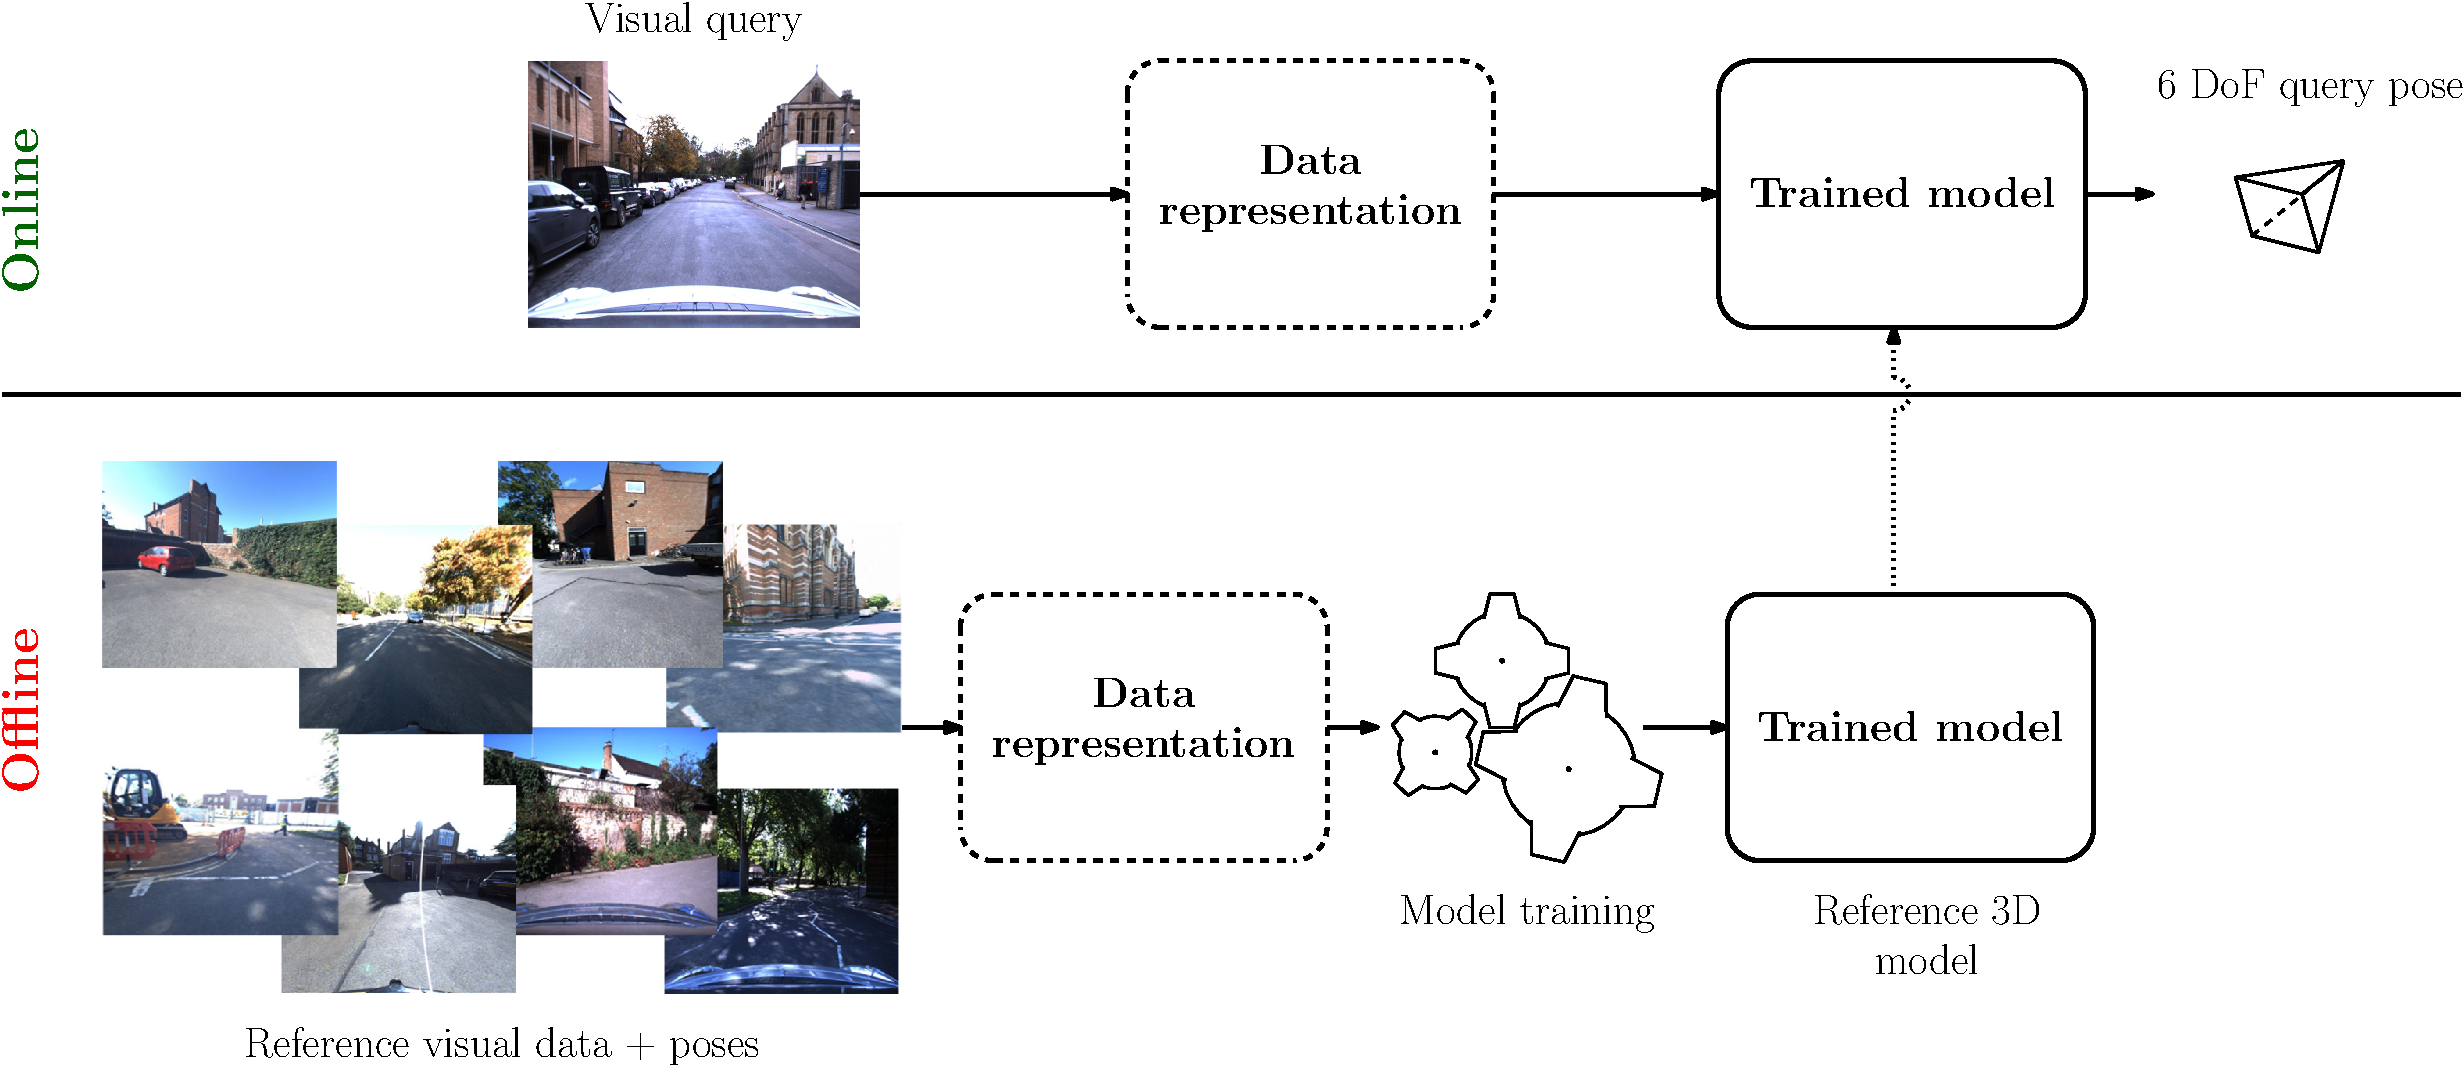
\includegraphics[width=\linewidth]{methods/learned_method}
	\caption[Learned method]{\label{fig:learned_method}\textbf{Learned method for \acs{vbl}:} a model is trained with geolocalized data in order to regress the right pose of a visual request. Once trained, the model is used to predict the pose of a unknown query. The data can be preprocessed (dotted blocks) before the evaluation by the model.}
\end{figure}
